\documentclass[]{mcom-l}


\usepackage{latexsym,amsfonts,amsmath,amssymb,amsthm,epsfig,extdash,multirow}
\usepackage{stackrel,tabularx,mathtools,enumitem,longtable,xspace}
\usepackage[dvipsnames]{xcolor}
%\usepackage[numbers,sort&compress]{natbib}
\usepackage{hyperref,accents, booktabs}
\usepackage{algorithm, algorithmicx}
\usepackage{anyfontsize}
\usepackage{cleveref}
\usepackage{wrapfig}
\usepackage[font=small,labelfont=bf]{caption}

\usepackage{algpseudocode}
\usepackage{algorithm, algorithmicx}
\algnewcommand\algorithmicparam{\textbf{Parameters:}}
\algnewcommand\PARAM{\item[\algorithmicparam]}
\algnewcommand\algorithmicinput{\textbf{Input:}}
\algnewcommand\INPUT{\item[\algorithmicinput]}
\algnewcommand\RETURN{\State \textbf{Return }}
\usepackage{algpseudocode}

\theoremstyle{remark}
\newtheorem{example}{Example}
%%list of acronyms with links
\newcommand{\QMCSoft}{QMCSoft\xspace}
\newcommand{\GAIL}{GAIL\xspace}
\newcommand{\QMC}{QMC\xspace}
\newcommand{\IIDMC}{IID MC\xspace}
\newcommand{\SAMSIQMC}{SAMSI-QMC\xspace}
\newcommand{\SciPy}{SciPy\xspace}
\newcommand{\GSL}{GSL\xspace}
\newcommand{\NAG}{NAG\xspace}
\newcommand{\MATLAB}{MATLAB\xspace}
\newcommand{\Chebfun}{Chebfun\xspace}
\newcommand{\Rlang}{R\xspace}
\newcommand{\Julia}{Julia\xspace}


\textwidth6.5in
\setlength{\oddsidemargin}{0in}
\setlength{\evensidemargin}{0in}
\textheight9.0in
%\textheight9.1in

\newtheorem{theorem}{theorem}


\providecommand{\FJHickernell}{Hickernell}
\newcommand{\hf}{\widehat{f}}
\newcommand{\hg}{\widehat{g}}
\newcommand{\hI}{\hat{I}}
\newcommand{\hatf}{\hat{f}}
\newcommand{\hatg}{\hat{g}}
\newcommand{\tf}{\widetilde{f}}
\newcommand{\tbf}{\tilde{\bff}}
\newcommand{\vBall}{\text{vBall}_n}
\newcommand{\vEll}{\text{vEll}}
%\DeclareMathOperator{\Pr}{\mathbb{P}}

% Math operators
%\DeclareMathOperator{\cost}{COST}
%\DeclareMathOperator{\comp}{COMP}
%\DeclareMathOperator{\loss}{loss}
%\DeclareMathOperator{\lof}{lof}
%\DeclareMathOperator{\reg}{reg}
%\DeclareMathOperator{\CV}{CV}
%\DeclareMathOperator{\size}{wd}
\DeclareMathOperator{\GP}{\mathcal{G} \! \mathcal{P}}
%\DeclareMathOperator{\erf}{erf}
\DeclareMathOperator*{\argmax}{arg\,max}
\DeclareMathOperator*{\argmin}{arg\,min}
%\DeclareMathOperator{\QOI}{QOI} %Quantity of Interest
%\DeclareMathOperator{\POI}{POI} %Parameter of Interest
%\DeclareMathOperator{\Ans}{ANS}
%\DeclareMathOperator{\Var}{Var}
%\DeclareMathOperator{\APP}{\widehat{\QOI}}
%\DeclareMathOperator{\SURR}{SM} %surrogate model
%\DeclareMathOperator{\STREND}{ST} %surrogate trend
%\DeclareMathOperator{\SVAR}{SV} %surrogate variation
%\DeclareMathOperator{\SVARERR}{SVU} %surrogate variation uncertainty
%\newcommand{\MLS}{\textrm{MLS}\xspace} %distance weighted least squares, also known as moving least squares
\DeclareMathOperator{\ALG}{ALG}
\DeclareMathOperator{\ACQ}{ACQ}
\DeclareMathOperator{\ERR}{ERR}
%\DeclareMathOperator{\VAL}{ACQ}
%\DeclareMathOperator{\OPER}{OPER}
%\DeclareMathOperator{\INT}{INT}
%\DeclareMathOperator{\MIN}{MIN}
%\DeclareMathOperator{\ID}{ID}
%\DeclareMathOperator{\APPMIN}{\widehat{\MIN}}
%\DeclareMathOperator{\APPID}{\widehat{\ID}}
%\DeclareMathOperator{\MINVAL}{MINACQ}
%\DeclareMathOperator{\IDVAL}{IDACQ}
%\DeclareMathOperator{\SURRERR}{SU}
%\DeclareMathOperator{\MINERR}{MERR}
%\DeclareMathOperator{\IDERR}{IDERR}
\DeclareMathOperator{\Prob}{\mathbb{P}}
\DeclareMathOperator{\diag}{diag}
%\DeclareMathOperator{\dist}{dist}
%\DeclareMathOperator{\filldis}{fill}
%\DeclareMathOperator{\sep}{sep}
%\DeclareMathOperator{\avg}{avg}
\DeclareMathOperator{\vol}{vol}
%\DeclareMathOperator{\cov}{cov}
\DeclareMathOperator{\APP}{APP}
\newcommand{\TREND}{\textup{T}}
\newcommand{\VAR}{\textup{V}}
\newcommand{\LS}{\textup{LS}}

\newcommand{\NT}{{N_{\mT}}}
\newcommand{\Ntheta}{{N_{\btheta}}}


\newcommand{\reals}{{\mathbb{R}}}
\newcommand{\naturals}{{\mathbb{N}}}
\newcommand{\natzero}{{\mathbb{N}_0}}
\newcommand{\integers}{{\mathbb{Z}}}
\def\expect{{\mathbb{E}}}
\def\il{\left \langle}
\def\ir{\right \rangle}
\def\e{\varepsilon}
\def\g{\gamma}
\def\l{\lambda}
\def\b{\beta}
\def\a{\alpha}
\def\lall{\Lambda^{{\rm all}}}
\def\lstd{\Lambda^{{\rm std}}}

\newcommand{\vf}{\boldsymbol{f}}
\newcommand{\hV}{\widehat{V}}
\newcommand{\tV}{\widetilde{V}}
\newcommand{\fraku}{\mathfrak{u}}
\newcommand{\hcut}{\mathfrak{h}}
\newcommand{\tOmega}{\widetilde{\Omega}}
\newcommand{\tvarrho}{\widetilde{\varrho}}

\newcommand{\bbE}{\mathbb{E}}
\newcommand{\tQ}{\widetilde{Q}}
\newcommand{\mA}{\mathsf{A}}
\newcommand{\mB}{\mathsf{B}}
\newcommand{\mC}{\mathsf{C}}
\newcommand{\mD}{\mathsf{D}}
\newcommand{\mG}{\mathsf{G}}
\newcommand{\mH}{\mathsf{H}}
\newcommand{\mI}{\mathsf{I}}
\newcommand{\bbK}{\mathbb{K}}
\newcommand{\mK}{\mathsf{K}}
\newcommand{\tmK}{\widetilde{\mathsf{K}}}
\newcommand{\mL}{\mathsf{L}}
\newcommand{\mM}{\mathsf{M}}
\newcommand{\mP}{\mathsf{P}}
\newcommand{\mQ}{\mathsf{Q}}
\newcommand{\mR}{\mathsf{R}}
\newcommand{\mT}{\mathsf{T}}
\newcommand{\mU}{\mathsf{U}}
\newcommand{\mX}{\mathsf{X}}
\newcommand{\mZero}{\mathsf{0}}
\newcommand{\mPhi}{\mathsf{\Phi}}
\newcommand{\mPsi}{\mathsf{\Psi}}
\newcommand{\mLambda}{\mathsf{\Lambda}}
\newcommand{\cube}{[0,1]^d}
\newcommand{\design}{\{\bx_i\}_{i=1}^n}




\newcommand{\bone}{\boldsymbol{1}}
\newcommand{\bzero}{\boldsymbol{0}}
\newcommand{\binf}{\boldsymbol{\infty}}
\newcommand{\ba}{{\boldsymbol{a}}}
\newcommand{\bb}{{\boldsymbol{b}}}
\newcommand{\bc}{{\boldsymbol{c}}}
\newcommand{\bd}{{\boldsymbol{d}}}
\newcommand{\be}{{\boldsymbol{e}}}
\newcommand{\bff}{{\boldsymbol{f}}}
\newcommand{\bhh}{{\boldsymbol{h}}}
\newcommand{\beps}{{\boldsymbol{\varepsilon}}}
\newcommand{\tbeps}{\tilde{\beps}}
\newcommand{\bx}{{\boldsymbol{x}}}
\newcommand{\bX}{{\boldsymbol{X}}}
\newcommand{\bh}{{\boldsymbol{h}}}
\newcommand{\bj}{{\boldsymbol{j}}}
\newcommand{\bk}{{\boldsymbol{k}}}
\newcommand{\vell}{{\boldsymbol{\ell}}}
\newcommand{\bL}{{\boldsymbol{L}}}
\newcommand{\bg}{{\boldsymbol{g}}}
\newcommand{\bn}{{\boldsymbol{n}}}
\newcommand{\bp}{{\boldsymbol{p}}}
\newcommand{\bP}{{\boldsymbol{P}}}
\newcommand{\br}{{\boldsymbol{r}}}
\newcommand{\bv}{{\boldsymbol{v}}}
\newcommand{\bu}{{\boldsymbol{u}}}
\newcommand{\by}{{\boldsymbol{y}}}
\newcommand{\bt}{{\boldsymbol{t}}}
\newcommand{\bU}{{\boldsymbol{U}}}
\newcommand{\bz}{{\boldsymbol{z}}}
\newcommand{\bvarphi}{{\boldsymbol{\varphi}}}
\newcommand{\bgamma}{{\boldsymbol{\gamma}}}
\newcommand{\bphi}{{\boldsymbol{\phi}}}
\newcommand{\bpsi}{{\boldsymbol{\psi}}}
\newcommand{\btheta}{{\boldsymbol{\theta}}}
\newcommand{\bnu}{{\boldsymbol{\nu}}}
\newcommand{\balpha}{{\boldsymbol{\alpha}}}
\newcommand{\bbeta}{{\boldsymbol{\beta}}}
\newcommand{\bo}{{\boldsymbol{\omega}}}  %GF added
\newcommand{\newton}[2]{\left(\begin{array}{c} #1\\ #2\end{array}\right)}
\newcommand{\anor}[2]{\| #1\|_{\mu_{#2}}}
\newcommand{\satop}[2]{\stackrel{\scriptstyle{#1}}{\scriptstyle{#2}}}
\newcommand{\setu}{{\mathfrak{u}}}

\newcommand{\me}{\textup{e}}
\newcommand{\mi}{\textup{i}}
\def\d{\textup{d}}
\def\dif{\textup{d}}
\newcommand{\cc}{\mathcal{C}}
\newcommand{\cb}{\mathcal{B}}
\newcommand{\cl}{L}
\newcommand{\ct}{\mathfrak{T}}
\newcommand{\cx}{{\Omega}}
\newcommand{\cala}{{\mathcal{A}}}
\newcommand{\calc}{{\mathcal{C}}}
\newcommand{\calf}{{\mathcal{F}}}
\newcommand{\calfd}{{\calf_d}}
\newcommand{\calh}{{\mathcal{H}}}
\newcommand{\tcalh}{{\widetilde{\calh}}}
\newcommand{\calI}{{\mathcal{I}}}
\newcommand{\calhk}{\calh_d(K)}
\newcommand{\calg}{{\mathcal{G}}}
\newcommand{\calgd}{{\calg_d}}
\newcommand{\caln}{{\mathcal{N}}}
\newcommand{\calp}{{\mathcal{P}}}
\newcommand{\cals}{{\mathcal{S}}}
\newcommand{\cL}{\mathcal{L}}
\newcommand{\cP}{\mathcal{P}}
\newcommand{\cT}{\mathcal{T}}
\newcommand{\cK}{\mathcal{K}}
\newcommand{\fA}{\mathfrak{A}}
\newcommand{\fC}{\mathfrak{C}}
\newcommand{\fF}{\mathfrak{F}}
\newcommand{\fL}{\mathfrak{L}}
\newcommand{\fU}{\mathfrak{U}}
\newcommand{\hS}{\widehat{S}}

\def\abs#1{\ensuremath{\left \lvert #1 \right \rvert}}
\newcommand{\bigabs}[1]{\ensuremath{\bigl \lvert #1 \bigr \rvert}}
\newcommand{\norm}[2][{}]{\ensuremath{\left \lVert #2 \right \rVert}_{#1}}
\newcommand{\ip}[3][{}]{\ensuremath{\left \langle #2, #3 \right \rangle_{#1}}}
\newcommand{\bignorm}[2][{}]{\ensuremath{\bigl \lVert #2 \bigr \rVert}_{#1}}
\newcommand{\Bignorm}[2][{}]{\ensuremath{\Bigl \lVert #2 \Bigr \rVert}_{#1}}
\newcommand{\calm}{{\mathfrak{M}}}

\newcommand{\des}{\{\bx_i\}}
\newcommand{\desinf}{\{\bx_i\}_{i=1}^{\infty}}
\newcommand{\desn}{\{\bx_i\}_{i=1}^n}
\newcommand{\wts}{\{g_i\}_{i=1}^N}
\newcommand{\wtsn}{\{g_i\}_{i=1}^N}
\newcommand{\datan}{\{y_i\}_{i=1}^N}

%FJH added
\newcommand{\Order}{\mathcal{O}}
\newcommand{\ch}{\mathcal{H}}
\newcommand{\tch}{{\widetilde{\ch}}}
\newcommand{\veps}{\boldsymbol{\varepsilon}}
\DeclareMathOperator{\best}{best}
\newcommand{\hmu}{\hat{\mu}}
\newcommand{\hsigma}{\hat{\sigma}}
\newcommand{\tK}{\widetilde{K}}
%\newcommand{\Matlab}{{\sc Matlab}\xspace}
\newcommand{\abstol}{\varepsilon_{\text{a}}}
\newcommand{\reltol}{\varepsilon_{\text{r}}}

\newcommand\starred[1]{\accentset{\star}{#1}}

\newcommand{\designInf}{\{\bx_i\}_{i=1}^\infty}
\newcommand{\dataN}{\bigl\{\bigl(\bx_i,f(\bx_i)\bigr)\bigr\}_{i=1}^n}
\newcommand{\dataNp}{\bigl\{\bigl(\bx_i,f(\bx_i)\bigr)\bigr\}_{i=1}^{n'}}
\newcommand{\dataNo}{\bigl\{\bigl(\bx_i,f(\bx_i)\bigr)\bigr\}_{i=1}^{n_0}}
\newcommand{\ErrN}{\ERR\bigl(\dataN,n\bigr)}
\newcommand{\fint}{f_{\text{int}}}
\newcommand{\inflate}{\fC}

\newcommand{\FredNote}[1]{{\color{blue}Fred: #1}}

\title{Adaptive Multivariate Sampling to Accelerate Discovery}
\author{}
\date{\today}

\begin{document}

\maketitle

\section{Introduction}
Rigorous error bounds for numerical approximations typically consist of the norm of the input function multiplied by the norm of the error operator.  Because the norm of the input function is unknown, these error bounds cannot tell us whether a prescribed error tolerance has been met.  Adaptive numerical algorithms typically use heuristic data-driven error bounds, which means that we don't know under what conditions they can be trusted.

We propose an adaptive function approximation algorithm based on rigorous, data-driven error bounds.  This algorithm assumes that the function to be approximated lies in a \emph{candidate cone}, $\cc$.  ``Candidate'' means those functions that our algorithm can approximate accurately.  The definition of $\cc$ formalizes the idea that \emph{what you observe is nearly what you get}.  If $f \in \cc$, then any constant multiple of $f$ is also in $\cc$, which makes $\cc$ a cone.  The underlying numerical approximation is the well-known reproducing kernel Hilbert space (RKHS) minimum norm interpolant with an explicit error bound.  Baking into $\cc$ the assumption that the norm of a function is not arbitrarily larger than the norm of its interpolant allows us to construct a rigorous adaptive function approximation algorithm. Given a black-box input function, $f$, and an error tolerance, $\varepsilon$, our algorithm returns an approximation, $\ALG(f,\varepsilon) \in L^\infty$---defined only in terms of function values---for which 
\begin{equation} \label{eq:errorcrit}
\norm[\infty]{f - \ALG(f,\varepsilon)} \le \varepsilon \qquad \forall f\in \cc.
\end{equation}

Adaption can take several forms, including
\begin{itemize}
    \item Adaptive choice of the number of function data needed, $n$, (Section \ref{sec:basicIdea}),
    \item Adaptive choice of the data sites, $\{\bx_1, \bx_2, \ldots\}$,  (Section \ref{sec:adaptSites}), and
    \item Adaptive choice of the function space, $\calf$, for which the input function is typical  (Section \ref{sec:adaptF}).
\end{itemize}
Algorithm \ref{alg:basicadapt} incorporates the idea of the candidate cone and the first kind of adaption.  Algorithm \ref{alg:adaptsample} adds the second kind of adaption, and Algorithm \ref{alg:adapttheta} adds the third kind of adaption.  Our theory is developed initially for functions lying purely in a RKHS.  In Section \ref{sec:poly} and Algorithm \ref{alg:poly} we generalize to the setting where a low-dimensional space of functions, e.g., polynomials of fixed degre, are exactly reproduced.

These algorithms draw upon the well-developed literature of RKHS function approximation \cite{Buh03a,Fas07a,FasMcC15a,ForFly15a,ForEtal09,RasWil06a,SchWen06a,Wah85a,Wen05a}.  Our main contributions are 
\begin{itemize}
	\item The candidate cone (Section \ref{sec:basicIdea}),
	\item A geometric interpretation of the condition to infer the suitable Hilbert space (Section  \ref{sec:adaptTheta}), and
	\item Inferring the location dependence of the reproducing kernel ( Section \ref{sec:InferSpace}) .
\end{itemize}

Any algorithm that claims to satisfy \eqref{eq:errorcrit} cannot possibly do so for a candidate set corresponding to an infinite dimensional vector space.  If there were such an algorithm, then $\ALG(0,\varepsilon)$ would terminate after evaluating the zero function at some $\bx_1, \ldots, \bx_n$.  Since $\cc$ is an infinite dimensional vector space, there exists some $g \in \cc$, for which $g(\bx_1) = \cdots = g(\bx_n) = 0$ but for which $\norm[\infty]{g} > 2 \varepsilon$.  That is, $g$ looks like $0$ to the algorithm, but is not close enough to $0$.  In this case, $\ALG(g,\varepsilon) = \ALG(0,\varepsilon)$, and it is impossible for the error criterion \eqref{eq:errorcrit} to be satisfied for both $f=0$ and $f = g$.

Function approximation algorithms are often constructed to satisfy error criterion \eqref{eq:errorcrit} for a candidate ball, e.g., $\cc = \{f \in \calf : \norm[\calf]{f} \le 1\}$.  Choosing this convex, symmetric candidate set guarantees that adaption is of no value \cite{Bak71}.  Here we choose candidate cones that are unbounded and non-convex, which are amenable to adaptive algorithms.

The algorithms constructed here put a premium on the cost of obtaining function values.  We have in mind the situation where one function value may be the result of an expensive simulation costing hours or days of CPU time, denoted $\$(f)$.  Our algorithm produces an inexpensive surrogate or approximation of the expensive simulation.  If $n$ function values are required to obtain a satisfactory function approximation, then we do not mind if the manipulation of that data to form our function approximation requires $\Order(n^p)$ operations, since practically speaking this will be smaller than $\$(f) n$.  RKHS minimum  norm interpolants typically require $\Order(n^3)$ operations, and we may require a bit more to obtain a satisfactory error bound.  Methods to reduce the computational effort required to construct RKHS minimum norm interpolants include an estimating equation approach \cite{AniCheSte16a}, approximation by incomplete Cholesky factorizations \cite{OwhEtal19a}, and matching designs with kernels to obtain Gram matrices that can be inverted using fast transforms \cite{RatHic19a}.




%%%%%%%%%%%%%%%%%%%%%%%%%%%%%%%%%%%%%%%%%%%%%%%%%%%%%%%%%%%%%%%%%%%%%%
%%%%%%%%%%%%%%%%%%%%%%%%%%%%%%%%%%%%%%%%%%%%%%%%%%%%%%%%%%%%%%%%%%%%%%
\section{Adaptive Function Approximation for a Fixed Hilbert Space} \label{sec:fixedF}
%%%%%%%%%%%%%%%%%%%%%%%%%%%%%%%%%%%%%%%%%%%%%%%%%%%%%%%%%%%%%%%%%%%%%%
%%%%%%%%%%%%%%%%%%%%%%%%%%%%%%%%%%%%%%%%%%%%%%%%%%%%%%%%%%%%%%%%%%%%%%

%%%%%%%%%%%%%%%%%%%%%%%%%%%%%%%%%%%%%%%%%%%%%%%%%%%%%%%%%%%%%%%%%%%%%%
%%%%%%%%%%%%%%%%%%%%%%%%%%%%%%%%%%%%%%%%%%%%%%%%%%%%%%%%%%%%%%%%%%%%%%
\subsection{The Basic Idea Our Adaptive Algorithm} \label{sec:basicIdea}
%%%%%%%%%%%%%%%%%%%%%%%%%%%%%%%%%%%%%%%%%%%%%%%%%%%%%%%%%%%%%%%%%%%%%%
%%%%%%%%%%%%%%%%%%%%%%%%%%%%%%%%%%%%%%%%%%%%%%%%%%%%%%%%%%%%%%%%%%%%%%
Suppose that $f$, belongs to an RKHS $\calf$ of functions with domain $\cx$.  Let $K: \Omega \times \Omega \to \reals$ denote the reproducing kernel.  Let $\mX = (\bx_1, \ldots, \bx_n)^T \in \cx^n \subseteq \reals^{n \times d}$ be an array of $n$ data sites, and let $\by  = f(\mX) \in \reals^n$ denote the array of function values at these data sites.  
The minimum norm interpolant of $f$ is 
\begin{subequations} \label{eq:RKHSAPP}
\begin{align} 
\APP(\mX,\by) &= \sum_{i=1}^n c_i K(\bx_i,\cdot) = \bc^T K(\mX,\cdot) =  K(\cdot, \mX) \mK^{-1} \by, \\
 \text{where } & \qquad \bc = \mK^{-1} \by, \quad \mK = K(\mX,\mX) = \bigl( K(\bx_i,\bx_j) \bigr)_{i,j=1}^n,  \\
& \qquad  K(\mX,\bx) = \bigl(K(\bx,\bx_i) \bigr)_{i=1}^n =  K(\bx, \mX)^T.
\end{align}
\end{subequations}
This has a known pointwise error bound of \cite{bibid}
\begin{align}
\label{eq:RKHSErrBd}
\abs{f(\bx) - \APP(\mX,\by)(\bx)} & \le \sqrt{K(\bx,\bx) - K(\bx,\mX) \mK^{-1} K(\mX,\bx)} \, \bignorm[\calf]{f - \APP(f)} \\
\nonumber
& \le \sqrt{K(\bx,\bx) - K(\bx,\mX) \mK^{-1} K(\mX,\bx) } \, \norm[\calf]{f} .
\end{align}

Data-based approximation $\APP(\mX,\by)$ in \eqref{eq:RKHSAPP} is an ingredient in our adaptive algorithm, but error bound \eqref{eq:RKHSErrBd} contains the unknown factor $\norm[\calf]{f - \APP(\mX,\by)}$, which cannot be computed from function data.  What we can compute from data is $\bignorm[\calf]{\APP(f)} = \sqrt{\by^T \mK^{-1} \by}$.  Moreover, it is known that the error is orthogonal to the approximation, so by the Pythagorean Theorem,  $\norm[\calf]{f}^2  = \bignorm[\calf]{\APP(f)}^2 + \bignorm[\calf]{f - \APP(f)}^2$.  To establish a data-driven error bound, we define a candidate cone
\begin{align} \label{eq:RKHScone}
\calc &:= \Bigl\{f \in \calf : \norm[\calf]{f}^2 \le (1 + A^2(\mX)) \bignorm[\calf]{\APP(\mX,\by)}^2 \quad \forall \mX \in \Omega^d, \ \by = f(\mX) \Bigr \} \\
\nonumber
& = \Bigl \{f \in \calf : \bignorm[\calf]{f - \APP(f)} \le A(\mX) \bignorm[\calf]{\APP(\mX,\by)} \quad \forall \mX \in \Omega^d, \ \by = f(\mX) \Bigr \} \\
\nonumber
& = \Bigl \{f \in \calf : \bignorm[\calf]{f - \APP(f)}^2 \le \frac{A^2(\mX)}{1 + A^2(\mX)} \bignorm[\calf]{f}^2 \quad \forall \mX \in \Omega^d, \ \by = f(\mX) \Bigr \},
\end{align}
where $A(\mX)$ is positive and fixed in advance. Larger $A(\mX)$ yields a more inclusive candidate cone.  This candidate set is a cone because if $f \in \calc$, then $c f \in \calc$ for any real $c$. 

The intuition that inspires our candidate cone is \emph{what you have not yet seen is not much worse than what you have seen}. All adaptive algorithms are based on this philosophy. The definition of the cone in \eqref{eq:RKHScone} is a way of formalizing this. 

Because $\bignorm[\calf]{\APP(\mX,\by)} = \sqrt{\by^T \mK^{-1} \by}$, error bound \eqref{eq:RKHSErrBd} implies an error bound that can be computed solely based on the function data: 
\begin{subequations} \label{eq:DataErrBd}
\begin{align}
\label{eq:DataErrBdA}
    \abs{f(\bx) - \APP(\mX,\by)(\bx)} & \le   A(\mX) \sqrt{[K(\bx,\bx) - K(\bx,\mX) \mK^{-1} K(\mX,\bx) ] \, [\by^T \mK^{-1} \by] } \qquad \forall f \in \calc, \\
    \label{eq:DataErrBdB}
    \norm[\infty]{f - \APP(\mX,\by)} & \le   A(\mX) \sqrt{\norm[\infty]{K(\cdot,\cdot) - K(\cdot,\mX) \mK^{-1} K(\mX,\cdot)} \, [\by^T \mK^{-1} \by] } \qquad \forall f \in \calc.
\end{align}
\end{subequations}
This data-based error bound provides what is needed for our adaptive algorithm.  Note that $n$ is implicit in the definition of $\mX$, but we do not show this explicitly to for notational simplicity.

\begin{algorithm}[H]
\caption{Adaptive Sample Size \label{alg:basicadapt}}
	\begin{algorithmic}
	\PARAM the RKHS, $\calf$; the factor, $A(\cdot)$, which defines  the candidate cone, $\cc$, in \eqref{eq:RKHScone};  a sequence of data sites, $\{\bx_1, \bx_2, \ldots \}$; an initial sample size, $n_0$
	\INPUT a black-box function, $f \in \cc$; an absolute error tolerance, $\varepsilon>0$

    \Ensure Error criterion $\norm[\infty]{f - \ALG(f,\varepsilon)} \le \varepsilon$

   \State Let $n \leftarrow n_0 -1$

\Repeat

\State Let $n \leftarrow n + 1$

\State Compute $\by$, $A(\mX)$, $K(\mX,\mX)$, and $K(\mX,\cdot)$

\Until $A(\mX) \sqrt{\norm[\infty]{K(\cdot,\cdot) - K(\cdot,\mX) \mK^{-1} K(\mX,\cdot)} \, [\by^T \mK^{-1} \by] }  \le \varepsilon$

\RETURN $\ALG(f,\varepsilon) = \APP(\mX,\by)$

\end{algorithmic}
\end{algorithm}

This algorithm adaptively chooses the sample size so that the error criterion must be satisfied for all functions in the candidate cone $\cc$.  For a well chosen design, $\norm[\infty]{K(\cdot,\cdot) - K(\cdot,\mX) \mK^{-1} K(\mX,\cdot)}$ tends to zero as $n$ increases.  A larger function yields larger function data $\by$, which implies that a larger sample size will be required to achieve the error criterion.

However, there are several deficiencies in this algorithm.  The choice of the design does not yet depend in on the function data.  There is no assurance that the RKHS specified by the choice of $K$ fits $f$.  There is also the matter of how to choose $A(\mX)$.  These matters are addressed in the coming sections.


%%%%%%%%%%%%%%%%%%%%%%%%%%%%%%%%%%%%%%%%%%%%%%%%%%%%%%%%%%%%%%%%%%%%%%
%%%%%%%%%%%%%%%%%%%%%%%%%%%%%%%%%%%%%%%%%%%%%%%%%%%%%%%%%%%%%%%%%%%%%%
\subsection{Choosing a Reasonable $A$?}
%%%%%%%%%%%%%%%%%%%%%%%%%%%%%%%%%%%%%%%%%%%%%%%%%%%%%%%%%%%%%%%%%%%%%%
%%%%%%%%%%%%%%%%%%%%%%%%%%%%%%%%%%%%%%%%%%%%%%%%%%%%%%%%%%%%%%%%%%%%%%

The candidate cone depends on the factor $A(\mX)$, which, according to \ref{eq:RKHScone}, reflects how much larger one expects $\bignorm[\calf]{f  - \APP(\mX,\by)}$ might be than $\bignorm[\calf]{\APP(\mX,\by)}$ is.  It is natural for $A(\mX)$ to depend  on the quality of the design and the number of data sites.  One measure of the quality of the design is 
\begin{equation} \label{eq:BX}
B(\mX) : = \frac{ \sup \{\norm[\infty]{f} :  \norm[\calf]{f}  \le 1 , \ f(\mX) = 0 \}   }  {\sup \{ \norm[\infty]{f}  : \norm[\calf]{f}  \le 1  \} }
= \sqrt{ \frac{\norm[\infty]{K(\cdot,\cdot) - K(\cdot,\mX) \mK^{-1} K(\mX,\cdot)}}{\norm[\infty]{K(\cdot,\cdot)}}} \le 1.
\end{equation}
As the sample size increases using well-placed data, $B(\mX)$ tends to zero.

The choice of $A(\mX)$ is  a value judgment.  We propose
\begin{equation} \label{eq:an}
A(\mX): = \begin{cases} \displaystyle
\frac{A_\infty B_0}{B_0 - B(\mX)}, & B(\mX) < B_0, \\
\infty, & B(\mX) \ge B_0.
\end{cases}
\end{equation}
The parameter $A_\infty > 0$ represents the limiting value of $A(\mX)$ as the design tends to perfection.  The parameter $B_0$ represents the maximum value of $B(\mX)$ for which one is willing to infer a bound on $\bignorm[\calf]{f  - \APP(\mX,\by)}$ in terms of $\bignorm[\calf]{\APP(\mX,\by)}$.  Making $A_\infty$ larger or $B_0$ smaller makes the candidate cone, $\cc$ more inclusive.

The parameter $n_0$ in Algorithm \ref{alg:basicadapt} can be chosen as the minimum sample size for which $B(\mX) < B_0$.  This leaves only the two parameters $A_\infty$ and $B_0$ as requiring default values or to be chosen by the user.

\begin{example}
	Here we use one 1-d example to illustrate it.
	
	A commonly used reproducing kernel is the following member of the Mat\'ern family:
	\begin{equation} \label{eq:MaternOne}
	K(\bt,\bx) = (1 +  \norm{\bt-\bx}) \exp(-\norm{\bt-\bx}),
	\end{equation}
	where $\norm{\cdot}$ denotes the Euclidean norm.
	We have \[f: x \mapsto \exp(-6x) \sin(8x+0.1) - 0.1.\]
	Consider the $n=10$ point design $\mX = (0, 0.1, \ldots, 0.6, 0.8, 0.9, 1)^T$
	
	
	
\end{example}



%%%%%%%%%%%%%%%%%%%%%%%%%%%%%%%%%%%%%%%%%%%%%%%%%%%%%%%%%%%%%%%%%%%%%%
%%%%%%%%%%%%%%%%%%%%%%%%%%%%%%%%%%%%%%%%%%%%%%%%%%%%%%%%%%%%%%%%%%%%%%
\subsection{Optimization Problems} \label{sec:Optim}
%%%%%%%%%%%%%%%%%%%%%%%%%%%%%%%%%%%%%%%%%%%%%%%%%%%%%%%%%%%%%%%%%%%%%%
%%%%%%%%%%%%%%%%%%%%%%%%%%%%%%%%%%%%%%%%%%%%%%%%%%%%%%%%%%%%%%%%%%%%%%

Algorithm \ref{alg:basicadapt} requires numerical optimization to  
approximate the sup-norms that appear in via the data-based error bound in \eqref{eq:DataErrBdB} and the definition of $B(\mX)$ in \eqref{eq:BX}.  Finding the locations of optima is required below in \eqref{eq:nextsample} for adaptively choosing the next data site and for adaptively choosing the correct kernel in \eqref{eq:thetEB} in Section \ref{sec:adaptF}.  We do not consider identifying the best numerical optimization algorithms for these purposes in this article but recognize it as a problem for further research.  

Moreover, these optimization problems do not require high accuracy answers.  Underestimating 
\[\norm[\infty]{K(\cdot,\cdot) - K(\cdot,\mX) \mK^{-1} K(\mX,\cdot)}\]
in  \eqref{eq:DataErrBdB} or  \eqref{eq:BX} by several percent does not lead to significant loss of accuracy or efficiency.  
In our numerical examples, we approximate this quantity by direct search:
\begin{equation} \label{eq:normappx}
\norm[\infty]{K(\cdot,\cdot) - K(\cdot,\mX) \mK^{-1} K(\mX,\cdot)} \approx \norm[\infty]{\diag\bigl(K(\mT,\mT) - K(\mT,\mX) \mK^{-1} K(\mX,\mT) \bigr)},
\end{equation}
where $\mT := (\bt_1, \ldots, \bt_\NT)^T \in \cx^\NT$ is a fixed array of test points.



%%%%%%%%%%%%%%%%%%%%%%%%%%%%%%%%%%%%%%%%%%%%%%%%%%%%%%%%%%%%%%%%%%%%%%
%%%%%%%%%%%%%%%%%%%%%%%%%%%%%%%%%%%%%%%%%%%%%%%%%%%%%%%%%%%%%%%%%%%%%%
\subsection{Computational Cost} \label{sec:compCost}
%%%%%%%%%%%%%%%%%%%%%%%%%%%%%%%%%%%%%%%%%%%%%%%%%%%%%%%%%%%%%%%%%%%%%%
%%%%%%%%%%%%%%%%%%%%%%%%%%%%%%%%%%%%%%%%%%%%%%%%%%%%%%%%%%%%%%%%%%%%%%
We explained in the introduction that we are primarily concerned with the computational cost of obtaining function data, but we will count the cost of our algorithms.  Explicitly showing the $n$ dependence, the sequence of data vectors, $\by_1, \ldots, \by_n$, cost $\$(f)n$, explicitly showing that the cost of a function value might be quite large.  The Cholesky decompositions of $\mK_1, \ldots, \mK_n$ and $\mK_1^{-1}, \ldots, \mK_n^{-1}$ can all be computed in $\Order(n^3)$ operations as shown in the appendix.  The quantity on the right side of \eqref{eq:normappx} can be computed recursively for $1, \ldots, n$ data sites using a total of $\Order\bigl( \NT n^2 \bigr)$ operations, as shown in the appendix.  

Thus, the computational cost of Algorithm \ref{alg:basicadapt} is
\begin{equation} \label{eq:compcostbasic}
\Order\bigl(\$(f)n + n^3 + \NT n^2 \bigr),
\end{equation}
where $n$ is the final number of data sites required.  Again, our intended application is that for which $\$(f)$ dominates $n^2$ and $\NT n$.  



%%%%%%%%%%%%%%%%%%%%%%%%%%%%%%%%%%%%%%%%%%%%%%%%%%%%%%%%%%%%%%%%%%%%%%
%%%%%%%%%%%%%%%%%%%%%%%%%%%%%%%%%%%%%%%%%%%%%%%%%%%%%%%%%%%%%%%%%%%%%%
\subsection{Adaptive Choice of Data Sites }  \label{sec:adaptSites}
%%%%%%%%%%%%%%%%%%%%%%%%%%%%%%%%%%%%%%%%%%%%%%%%%%%%%%%%%%%%%%%%%%%%%%
%%%%%%%%%%%%%%%%%%%%%%%%%%%%%%%%%%%%%%%%%%%%%%%%%%%%%%%%%%%%%%%%%%%%%%

Algorithm \ref{alg:basicadapt} makes no use of data to choose the next data site.  It makes sense to choose the next data site where the pointwise error bound of the present approximation in \eqref{eq:RKHSErrBd} is greatest.  This corresponds to maximizing a data-based acquisition function, $\ACQ(\mX,\by)$:
\begin{subequations} \label{eq:nextsample}
\begin{gather} 
\bx_1 \text{ given}, \\
 \bx_{n+1} = \argmax_{\bx \in \Omega} \ACQ(\mX,\by)(\bx), \; n \in \naturals,  \qquad \ACQ(\mX,\by)(\bx) := K(\bx,\bx) - K(\bx,\mX)^T \mK^{-1} K(\mX,\bx).
\end{gather}
\end{subequations}
As was suggested in Section \ref{sec:compCost}, we can approximate this by a direct search
\begin{equation} \label{eq:nextsampleAPPX}
\bx_{n+1} \approx \argmax_{\bt_1, \ldots, \bt_\NT} \ACQ(\mX,\by)(\bt)
\end{equation}
where $\ACQ(\mX,\by)(\mT) = \diag\bigl(K(\mT,\mT) - K(\mT,\mX) \mK^{-1} K(\mX,\mT) \bigr)$.  

Under this adaptive choice of data sites in  \eqref{eq:nextsample} one may then choose $n_0 = 1$.  The improvement of Algorithm \ref{alg:basicadapt} becomes the following. 

\begin{algorithm}[H]
	\caption{Adaptive Data Site Selection and Adaptive Sample Size \label{alg:adaptsample}}
	\begin{algorithmic}
		\PARAM the RKHS, $\calf$; $A_\infty$ and $B_0$, which define  the candidate cone, $\cc$, in \eqref{eq:RKHScone}; an initial data site, $\bx_1$
		\INPUT a black-box function, $f \in \cc$; an absolute error tolerance, $\varepsilon>0$
		
		\Ensure Error criterion $\norm[\infty]{f - \ALG(f,\varepsilon)} \le \varepsilon$
		
		\State Let $n \leftarrow 0$
		
		\Repeat
		
		\If{ $n > 0$}
		
		\State Let $ \bx_{n+1} = \displaystyle \argmax_{\bx \in \Omega} [K(\bx,\bx) - K(\bx,\mX)^T \mK^{-1} K(\mX,\bx)]$
		
		\EndIf
		
		\State Let $n \leftarrow n + 1$
		
		\State Compute $\by$, $A(\mX)$, $\mK = K(\mX,\mX)$, and $K(\mX,\cdot)$
		
		\Until $A(\mX) \sqrt{\norm[\infty]{K(\cdot,\cdot) - K(\cdot,\mX) \mK^{-1} K(\mX,\cdot)} \, [\by^T \mK^{-1} \by] }  \le \varepsilon$
		
		\RETURN $\ALG(f,\varepsilon) = \APP(\mX,\by)$
		
	\end{algorithmic}
\end{algorithm}

Algorithm \ref{alg:adaptsample} has asymptotically the same cost as Algorithm \ref{alg:basicadapt}, which is given in \eqref{eq:compcostbasic}.  The cost of optimizing the acquisition function is the same as evaluating the error bound.

Unfortunately, the acquisition function defined in \eqref{eq:nextsample} does not yet depend on the function data, $\by$, but only on the data sites, $\mX$.  In that sense, this algorithm chooses data sites to fill gaps between data sites.  It cannot choose data sites more densely where the function  fluctuates more.  In the next section we improve our algorithm to make the acquisition function strongly dependent on $\by$.





%%%%%%%%%%%%%%%%%%%%%%%%%%%%%%%%%%%%%%%%%%%%%%%%%%%%%%%%%%%%%%%%%%%%%%%%%%
%%%%%%%%%%%%%%%%%%%%%%%%%%%%%%%%%%%%%%%%%%%%%%%%%%%%%%%%%%%%%%%%%%%%%%%%%%
\section{Function Approximation when the Hilbert Space Is Inferred} \label{sec:adaptF}
%%%%%%%%%%%%%%%%%%%%%%%%%%%%%%%%%%%%%%%%%%%%%%%%%%%%%%%%%%%%%%%%%%%%%%%%%%
%%%%%%%%%%%%%%%%%%%%%%%%%%%%%%%%%%%%%%%%%%%%%%%%%%%%%%%%%%%%%%%%%%%%%%%%%%



%%%%%%%%%%%%%%%%%%%%%%%%%%%%%%%%%%%%%%%%%%%%%%%%%%%%%%%%%%%%%%%%%%%%%%
%%%%%%%%%%%%%%%%%%%%%%%%%%%%%%%%%%%%%%%%%%%%%%%%%%%%%%%%%%%%%%%%%%%%%%
\subsection{Inferring the Parameters Defining the Reproducing Kernel} \label{sec:adaptTheta}
%%%%%%%%%%%%%%%%%%%%%%%%%%%%%%%%%%%%%%%%%%%%%%%%%%%%%%%%%%%%%%%%%%%%%%
%%%%%%%%%%%%%%%%%%%%%%%%%%%%%%%%%%%%%%%%%%%%%%%%%%%%%%%%%%%%%%%%%%%%%%

Until now, we have assumed a fixed RKHS.  However, unless there is strong a priori knowledge about the function to be approximated, $f$, there is no way to know whether $f$ is typical for  that RKHS.  We do not expect a unique RKHS for which $f$ is typical, but we want to infer a suitable RKHS from the data.  

Let $\{\calf_{\btheta} : \btheta \in \Theta\}$ be a family of RKHSs parameterized by $\btheta$.  An example is a generalization of the Mat\'ern kernel  in \eqref{eq:MaternOne}:
\begin{equation} \label{eq:MaternTheta}
K_\btheta(\bt,\bx) = (1 +  \norm{\btheta \odot (\bt-\bx)}) \exp(-\norm{\btheta \odot (\bt-\bx)}),
\end{equation}
where $\odot$ denotes the Hadamard or term-by-term product.  From this section forward, we highlight the dependence of the reproducing kernel, the function approximation, and related quantities on $\btheta$.

Let $\vBall$ denote the volume of a unit ball in $n$ dimensions, and let $\vEll(\btheta,\mX,\by)$ denote the volume of the ellipsoidal solid in $\reals^n$ consisting of all possible function data whose minimum-norm interpolants have an $\calf_{\btheta}$-norm no greater than that of the observed interpolant:
\begin{align*}
\vEll(\btheta,\mX,\by) &= \vol\bigl(\{ \bz \in \reals^n : \norm[\calf_{\btheta}]{\APP_{\btheta}(\mX,\bz)}  \le \norm[\calf_{\btheta}]{\APP_{\btheta}(\mX,\by)} \} \bigr) \\
& = \vol\Bigl( \bigl \{ \bz \in \reals^n : \bz^T \mK_\btheta^{-1} \bz \le \by^T \mK_\btheta^{-1} \by  \bigr \} \Bigr) \\
& = \vBall \sqrt{\det(\mK_{\btheta})  \, [\by^T \mK_\btheta^{-1} \by]^n } \qquad \text{by \cite{bibid}}
\end{align*}

The volume of the ellipsoidal solid, $\vEll(\btheta,\mX,\by)$, is a measure of how large the observed function data is with respect to the Hilbert space $\calf_{\btheta}$.  This measure is independent of the vertical scale of the reproducing kernel.  It does not change if the reproducing kernel $K_\btheta$ is replaced by $cK_{\btheta}$ for any positive constant $c$.  

Figure \ref{fig:ellipPlot} displays the one-dimensional Mat\'ern kernel in \eqref{eq:MaternTheta} for three different values of $\btheta = \theta$ and the corresponding  ellipsoidal solids $\{ \bz \in \reals^n : \bz^T \mK_\btheta^{-1} \bz \le \by^T \mK_\btheta^{-1} \by  \bigr \}$  defined for a two-sample design.  Here, $\theta = 2$ has the smallest volume (area).


\begin{figure}[H]
	\centering
	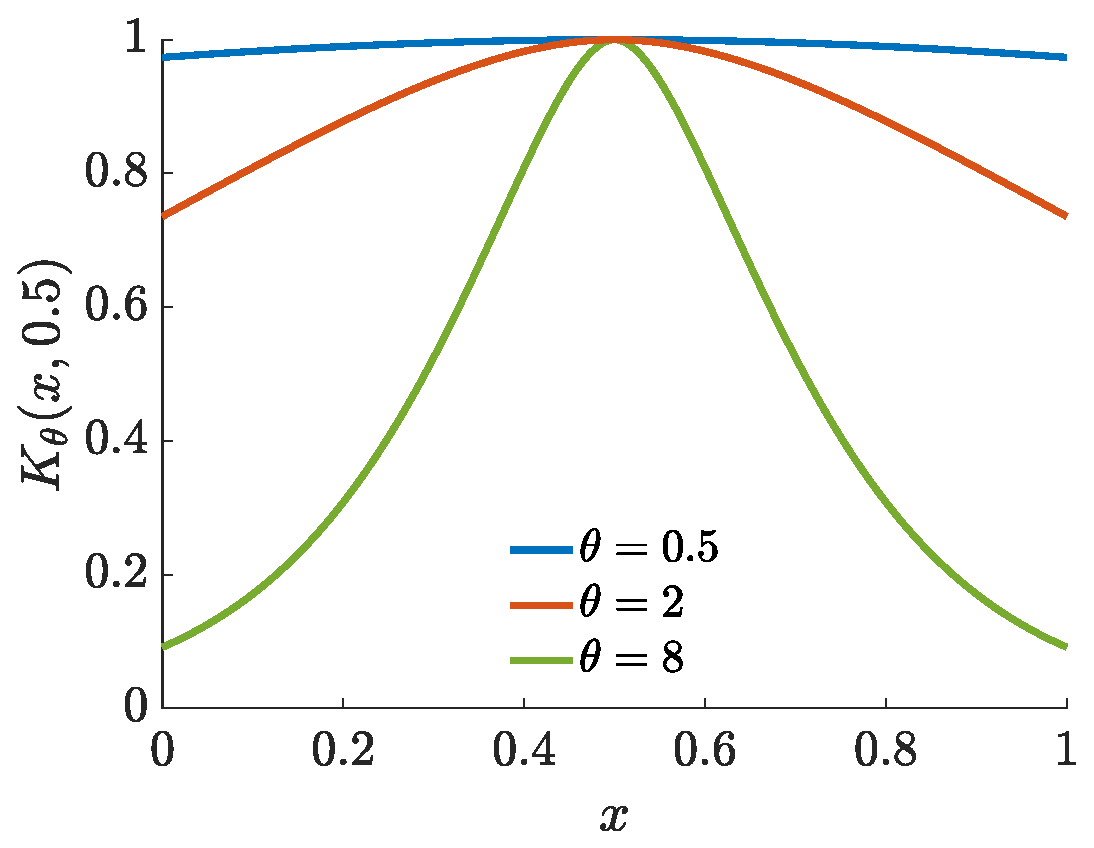
\includegraphics[height = 6cm]{ProgramsImages/KthetaPlot.eps} \qquad
	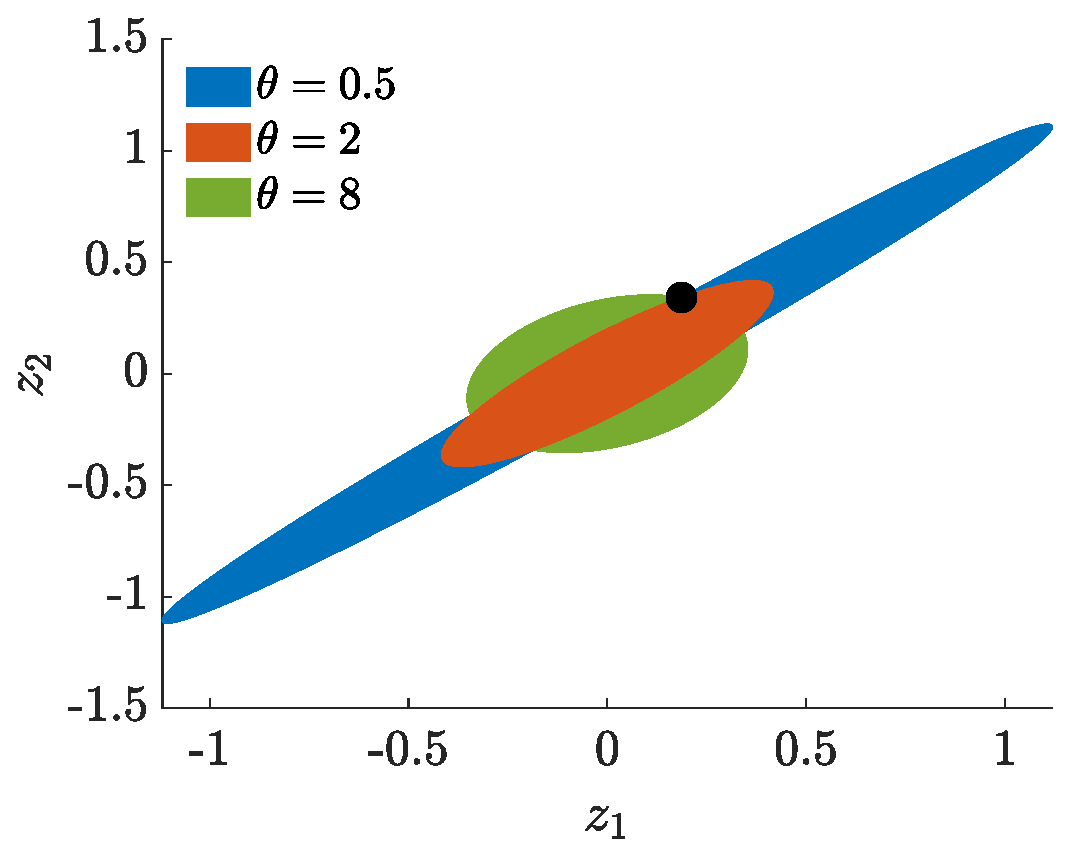
\includegraphics[height = 6cm]{ProgramsImages/ellipsesPlot.eps}
	\caption{The ellipsoidal solids $\{ \bz \in \reals^n : \bz^T \mK_\btheta^{-1} \bz \le \by^T \mK_\btheta^{-1} \by  \bigr \}$ for the Mat\'ern kernel defined in \eqref{eq:MaternTheta}, various values of $\btheta$, and $\by = f(\mX)$, where $\mX = (0.3 0.6)^T$ and $f$ is defined in ?? \label{fig:ellipPlot}}
\end{figure}

The reproducing kernel describes how large function values may be and how far apart two values of a function at different locations may be:
\begin{equation} \label{eq:diff_f}
\sup_{\norm[\calf_{\btheta}]{f} \le 1} \abs{f(\bx)}^2 = K(\bx,\bx), \qquad    \sup_{\norm[\calf_{\btheta}]{f} \le 1} \abs{f(\bt) - f(\bx)}^2 = K_{\btheta}(\bt,\bt) K_{\btheta}(\bx\bx) - 2 [K_{\btheta}(\bt,\bx)]^2.
\end{equation}
For the Mat\'ern kernel in \eqref{eq:MaternTheta} this corresponds to 
\begin{equation} \label{eq:diff_f_Matern}
\sup_{\norm[\calf_{\btheta}]{f} \le 1} \abs{f(\bx)}^2 = 1, \qquad 
\sup_{\norm[\calf_{\btheta}]{f} \le 1} \abs{f(\bt) - f(\bx)}^2 = 1 - 2 [(1 +  \norm{\btheta \odot (\bt-\bx)}) \exp(-\norm{\btheta \odot (\bt-\bx)})]^2.
\end{equation}
The Mat\'ern kernel with small $\theta$ is relatively flat, which means that function values in this RKHS do not vary much with location.  This explains why the ellipsoidal solid for $\theta = 0.5$ hugs the line $z_1 = z_2$.  For large $\theta$ the Mat\'ern kernel is peaked, which explains why the ellipsoidal solid for $\theta = 8$ is more spherical in shape.



We argue that the most suitable kernel is the one that minimizes the volume of the ellipsoidal solid, i.e., the RKHS for which the observed function data is small.   Our choice of $\btheta$ is
\begin{equation} \label{eq:thetEB}
\btheta  =  \argmin_{\theta'}  \vEll(\btheta' ,\mX,\by) 
 = \argmin_{\theta'}  \left[\frac 1n \log \bigl( \det(\mK_{\btheta'}) \bigr) + \log \bigl ( \by^T \mK_{\btheta'}^{-1} \by \bigr)\right].
\end{equation}

Inferring the reproducing kernel from the data necessitates a new candidate cone of functions to be approximated:
\begin{align} \label{eq:RKHSconeTheta}
\calc &: = \biggl \{f \in \bigcup_{\btheta' \in \Theta} \calf_{\btheta'} : \bignorm[\calf]{f - \APP_{\btheta}(f)} \le A_{\btheta}(\mX) \bignorm[\calf]{\APP_{\btheta}(\mX,\by)} \quad \forall \mX \in \Omega^d, \ \by = f(\mX) \\
& \hspace{8cm} \text{where $\btheta$ is selected by \eqref{eq:thetEB}} \biggr \}.
\nonumber
\end{align}
This candidate cone is neither a subset or superset of the candidate cone defined in \eqref{eq:RKHScone}.  Since it includes elements of multiple RKHSs, this new candidate cone is not a subset of the earlier one.  On the other hand, the condition that  the norm of the error of our approximation is bounded by the norm of the approximation for whatever $\btheta$ our criterion selects is a stricter condition than what is required in \eqref{eq:RKHScone}. 


\begin{algorithm}[H]
	\caption{Adaptive Data Site and RKHS Selection and Adaptive Sample Size \label{alg:adapttheta}}
	\begin{algorithmic}
		\PARAM the family of RKHSs, $\{\calf_{\btheta} : \btheta \in \Theta\}$; $A_\infty$ and $B_0$, which define the candidate cone, $\cc$, in \eqref{eq:RKHSconeTheta}; an initial data site, $\bx_1$
		\INPUT a black-box function, $f \in \cc$; an absolute error tolerance, $\varepsilon>0$
		
		\Ensure Error criterion $\norm[\infty]{f - \ALG(f,\varepsilon)} \le \varepsilon$
		
		\State Let $n \leftarrow 0$
		
		\Repeat
		
		\If{ $n > 0$}
		
		\State Let $ \bx_{n+1} = \displaystyle \argmax_{\bx \in \Omega} [K_\btheta(\bx,\bx) - K_\btheta(\bx,\mX)^T \mK_\btheta^{-1} K_\btheta(\mX,\bx)]$
		
		\EndIf
		
		\State Let $n \leftarrow n + 1$
		
		\State Update $\displaystyle\btheta = \argmin_{\theta'}  \left[\frac 1n \log \bigl( \det(\mK_{\btheta'}) \bigr) + \log \bigl ( \by^T \mK_{\btheta'}^{-1} \by \bigr)\right]$
		
		\State Compute $\by$, $A_\btheta(\mX)$, $\mK_\btheta = K_\btheta(\mX,\mX)$, and $K_\btheta(\mX,\cdot)$
		
		\Until $A_\btheta(\mX) \sqrt{\norm[\infty]{K_\btheta(\cdot,\cdot) - K_\btheta(\cdot,\mX) \mK_\btheta^{-1} K_\btheta(\mX,\cdot)} \, [\by^T \mK_\btheta^{-1} \by] }  \le \varepsilon$
		
		\RETURN $\ALG(f,\varepsilon) = \APP_\btheta(\mX,\by)$
		
	\end{algorithmic}
\end{algorithm}

Because $\btheta$ must be chosen by optimization, the asymptotic computational cost of Algorithm \ref{alg:adapttheta} is more than the earlier two algorithms.  Let $\Ntheta$ denote the number of $\btheta'$ values that must be tried at each step in the algorithm to obtain the optimum, $\btheta$.  The objective function for this optimization requires $\Order(n^3)$ operations to evaluate.  Moreover, since $\btheta$ may change for each $n$, the data-based error bound in the stopping criterion requires an evaluation of the sup-norm from scratch.  Therefore, the total cost of the algorithm is 
\begin{equation} \label{eq:compcosttheta}
\Order\bigl(\$(f)n + \Ntheta n^4 + \NT n^3 \bigr),
\end{equation}
where $n$ is the final number of data sites required.  Again, our intended application is that for which $\$(f)$ dominates $\Ntheta n^3$ and $\NT n^2$.  

\FredNote{Example again. Show how inferring $\btheta$ helps.}

%%%%%%%%%%%%%%%%%%%%%%%%%%%%%%%%%%%%%%%%%%%%%%%%%%%%%%%%%%%%%%%%%%%%%%
%%%%%%%%%%%%%%%%%%%%%%%%%%%%%%%%%%%%%%%%%%%%%%%%%%%%%%%%%%%%%%%%%%%%%%
\subsection{A Bayesian Numerical Analysis Digression} \label{sec:Bayes}
%%%%%%%%%%%%%%%%%%%%%%%%%%%%%%%%%%%%%%%%%%%%%%%%%%%%%%%%%%%%%%%%%%%%%%
%%%%%%%%%%%%%%%%%%%%%%%%%%%%%%%%%%%%%%%%%%%%%%%%%%%%%%%%%%%%%%%%%%%%%%

and the related Gaussian process modeling \cite{Dia88a,RasWil06a,Ste99}



%%%%%%%%%%%%%%%%%%%%%%%%%%%%%%%%%%%%%%%%%%%%%%%%%%%%%%%%%%%%%%%%%%%%%%
%%%%%%%%%%%%%%%%%%%%%%%%%%%%%%%%%%%%%%%%%%%%%%%%%%%%%%%%%%%%%%%%%%%%%%
\subsection{Inferring the Location Dependence of the Reproducing Kernel} \label{sec:InferSpace}
%%%%%%%%%%%%%%%%%%%%%%%%%%%%%%%%%%%%%%%%%%%%%%%%%%%%%%%%%%%%%%%%%%%%%%
%%%%%%%%%%%%%%%%%%%%%%%%%%%%%%%%%%%%%%%%%%%%%%%%%%%%%%%%%%%%%%%%%%%%%%

Although the function data, $\by$, appears in the selection criterion for $\btheta$, the form of reproducing kernel that we have considered thus far does not allow us to deduce that the function may vary more in one part of the domain than another.  The adaptive design defined by \eqref{eq:nextsample} may still be a space-filling design only slightly influenced by the observed function data.

\FredNote{Insert Example}

In the example above the function oscillates more on the left than the right, but \eqref{eq:diff_f_Matern} for the Mat\'ern kernel says that the maximum difference between function values at two locations is only a function of the distance between the locations.  The same holds for all $K(\bt ,\bx)$ that are  functions of $\bt - \bx$, i.e., the difference between the arguments.  Even for kernels that are not functions of the difference between the arguments, we would like to infer their location dependence from the data.

Given any reproducing kernel, $K(\bt ,\bx)$, it follows that $w(\bt)w(\bx)K(\bt ,\bx)$ is also a reproducing kernel for any function $w$.  Starting with the Mat\'ern kernel in \eqref{eq:MaternTheta}, we can generalize it further as follows:
\begin{align} \label{eq:MaternAB}
K_\btheta(\bt,\bx) &= \exp(\bb^T(\bt + \bx))(1 +  \norm{\ba \odot (\bt-\bx)}) \exp(-\norm{\ba \odot (\bt-\bx)}),  \quad \btheta=(\ba, \bb), \\
\nonumber
%\label{eq:diff_f_MaternAB}
\sup_{\norm[\calf_{\btheta}]{f} \le 1} \abs{f(\bx)}^2 &= \exp(2\bb^T\bx), \\
\nonumber
\MoveEqLeft[4]{\sup_{\norm[\calf_{\btheta}]{f} \le 1} \abs{f(\bt) - f(\bx)}^2} = \\
\nonumber 
& \qquad \exp(2\bb^T(\bt + \bx))\{ 1 - 2 (1 +  \norm{\ba \odot (\bt-\bx)}) \exp(-\norm{\ba \odot (\bt-\bx)})]^2\}.
\end{align}
For this kernel, the size of the function value and the difference between function values at different locations can generally rise or fall depending on the parameter $\bb$.


\FredNote{Repeat Example with new kernel}

%%%%%%%%%%%%%%%%%%%%%%%%%%%%%%%%%%%%%%%%%%%%%%%%%%%%%%%%%%%%%%%%%%%%%%
%%%%%%%%%%%%%%%%%%%%%%%%%%%%%%%%%%%%%%%%%%%%%%%%%%%%%%%%%%%%%%%%%%%%%%
\section{Recovering Low Degree Polynomials Exactly} \label{sec:poly}
%%%%%%%%%%%%%%%%%%%%%%%%%%%%%%%%%%%%%%%%%%%%%%%%%%%%%%%%%%%%%%%%%%%%%%
%%%%%%%%%%%%%%%%%%%%%%%%%%%%%%%%%%%%%%%%%%%%%%%%%%%%%%%%%%%%%%%%%%%%%%

The algorithm developed so far must be extended to recover even constant functions exactly.  Let $\calf_0$ be a finite dimensional vector space with basis $\{p_1, \ldots, p_s\}$.  For example, it might be space of polynomials.  To recover all functions in $\calf_0$ exactly, we modify our approximation in \eqref{eq:RKHSAPP} to take the form 
\begin{subequations} \label{eq:RKHSAPP_P}
	\begin{align} 
	\APP_\btheta(\mX,\by) &= \sum_{i=1}^n c_i K_\btheta(\bx_i,\cdot) + \sum_{j=1}^s \gamma_i p_j = \bc^T K_\btheta(\mX,\cdot) + \bgamma^T \bp(\cdot), \\
	\text{where } & \qquad \begin{pmatrix} \bc \\ \bgamma \end{pmatrix} = 
	\begin{pmatrix} \mK_\btheta  & \mP \\ \mP^T & \mZero_s \end{pmatrix}^{-1} 
	\begin{pmatrix}\by \\ \bzero_s \end{pmatrix}, 
	\quad \mK_\btheta = K_\btheta(\mX,\mX) = \bigl( K_\btheta(\bx_i,\bx_j) \bigr)_{i,j=1}^n,  \\
	& \qquad  K_\btheta(\mX,\bx) = \bigl(K_\btheta\bx,\bx_i) \bigr)_{i=1}^n =  K_\btheta(\bx, \mX)^T, \quad \mP = \bp^T(\mX) = \bigl( p_j(\bx_i)\bigr )_{i,j=1}^{n,s}.
	\end{align}
\end{subequations}
For any design $\mX$ and function data $\by$, let $\calg_\btheta(\mX,\by)$ denote the subset of $\calh_\btheta = \calf_0 \oplus \calf_\btheta$ that interpolates the data, i.e., $\calg_\btheta(\mX,\by) := \{ g = g_0 + g_{\btheta} : g_0 \in \calf_0, \ g_{\btheta} \in \calf_{\btheta}, \ g(\mX)  = \by\}$.  Moreover, defined a semi-norm for $\calf_0 \oplus \calf_\btheta$ as follows:
\begin{equation}
\abs{f}_{\calh_\btheta} = \min \{ \norm[\calf_\btheta] {f_\btheta} : f = f_0 + f_\btheta, \ f_0 \in \calf_0, \ f_\btheta \in \calf_\btheta \}
\end{equation}
Then, $\APP_\btheta(\mX,\by) = \argmin_{g \in \calg(\mX,\by)}  \abs{g}_{\calh_\btheta}$.

We assume that $\mP$ has full rank and that $\mK$ is invertible. Then
\begin{equation}
\bc = \mM_\btheta \by, \quad \mM_\btheta := \mK_\btheta^{-1} - \mK_\btheta^{-1}\mP (\mP^T \mK_\btheta^{-1} \mP)^{-1} \mP^T \mK_\btheta^{-1}, \qquad
\bgamma = (\mP^T \mK_\btheta^{-1} \mP)^{-1} \mP^T \mK_\btheta^{-1} \by.
\end{equation}
Then the error bound for $\APP_\btheta(\mX,\by)$ in \eqref{eq:RKHSErrBd} is extended to become
\begin{align}
\label{eq:RKHSErrBdP}
\abs{f(\bx) - \APP(\mX,\by)(\bx)} & \le \sqrt{K_\btheta(\bx,\bx) - K_\btheta(\bx,\mX) \mM_\btheta K_\btheta(\mX,\bx)} \, \bignorm[\calf_\btheta]{f - \APP(f)}.
\end{align}







\FredNote{Summary Theorem}
%%%%%%%%%%%%%%%%%%%%%%%%%%%%%%%%%%%%%%%%%%%%%%%%%%%%%%%%%%%%%%%%%%%%%%
%%%%%%%%%%%%%%%%%%%%%%%%%%%%%%%%%%%%%%%%%%%%%%%%%%%%%%%%%%%%%%%%%%%%%%
\section{Numerical Experiments}
%%%%%%%%%%%%%%%%%%%%%%%%%%%%%%%%%%%%%%%%%%%%%%%%%%%%%%%%%%%%%%%%%%%%%%
%%%%%%%%%%%%%%%%%%%%%%%%%%%%%%%%%%%%%%%%%%%%%%%%%%%%%%%%%%%%%%%%%%%%%%

\bibliographystyle{amsplain}
\bibliography{FJHown23,FJH23}

%%%%%%%%%%%%%%%%%%%%%%%%%%%%%%%%%%%%%%%%%%%%%%%%%%%%%%%%%%%%%%%%%%%%%%
%%%%%%%%%%%%%%%%%%%%%%%%%%%%%%%%%%%%%%%%%%%%%%%%%%%%%%%%%%%%%%%%%%%%%%
\section*{Appendix}
%%%%%%%%%%%%%%%%%%%%%%%%%%%%%%%%%%%%%%%%%%%%%%%%%%%%%%%%%%%%%%%%%%%%%%
%%%%%%%%%%%%%%%%%%%%%%%%%%%%%%%%%%%%%%%%%%%%%%%%%%%%%%%%%%%%%%%%%%%%%%
The Gram matrix, $\mK$ defined in \eqref{eq:RKHSAPP} is positive definite, and therefore has a Cholesky decomposition, $\mK = \mL \mD \mL^T$, where $\mL$ is a lower unitriangular matrix and $\mD$ is a diagonal matrix with positive diagonal elements.  Moreover, $\mK^{-1} = \mU \mD^{-1} \mU^T$, where $\mU := \mL^{-T}$ is an upper unitriangular matrix. As the sample size grows, these matrices can be constructed recursively.  Expressing the sample size $n$ in the notation, we claim that 
\begin{subequations} \label{eq:cholrecurse}
\begin{gather}
\label{eq:cholrecurseA}
\mK_1  = \mD_1 = K(\bx_1,\bx_1), \qquad \mL_1 = \mU_1 = 1,  \quad \\
\intertext{and for $n = 1, 2, \ldots$ we have recursively}
\label{eq:cholrecurseB}\mK_{n+1} = \begin{pmatrix}
\mK_n & K(\mX_n, \bx_{n+1}) \\
K(\bx_{n+1}, \mX_n) & K(\bx_{n+1}, \bx_{n+1})
\end{pmatrix},
\qquad 
\mD_{n+1} = \begin{pmatrix}
\mD_n & \bzero_n \\
\bzero_n^T & d_{n+1}
\end{pmatrix},
\\
\label{eq:cholrecurseC}
\mL_{n+1} = \begin{pmatrix}
\mL_n & \bzero_n \\
\bL_{n+1}^T  & 1
\end{pmatrix},
\qquad 
\mU_{n+1} = \begin{pmatrix}
\mU_n & \bU_{n+1} \\
\bzero_n^T  & 1
\end{pmatrix}, \\
\intertext{where}
\label{eq:cholrecurseD}
\vell_{n+1} = \mU_n^T K(\mX_n, \bx_{n+1}), \qquad
\bL_{n+1} = \mD_n^{-1} \vell_{n+1}, 
\\
\label{eq:cholrecurseE}
d_{n+1} = K(\bx_{n+1}, \bx_{n+1}) - \vell^T_{n+1} \bL_{n+1}, \qquad
\bU_{n+1} = - \mU_n \bL_{n+1}.
\end{gather}
\end{subequations}

The proof is by induction.  Certain properties follow automatically: the $n = 1$ case,  the recursive form for $\mK_{n+1}$, and the facts that $\mL_n$ is lower unitriangular, the $\mU_n$ is upper unitriangular, and $\mD_n$ is diagonal.  What need to be established are that $\mU_{n+1}= \mL^{-T}_{n+1}$ and that $\mK_{n+1} =  \mL_{n+1} \mD_{n+1} \mL^T_{n+1}$.   Given that  the formulas for $\mD_n$, $\mL_n$, and $\mU_n$ are correct, it follows that 
\begin{align*}
 \mU_{n+1} \mL_{n+1}^T & = 
 \begin{pmatrix}
 \mU_n & \bU_{n+1} \\
 \bzero_n^T  & 1
 \end{pmatrix}
 \begin{pmatrix}
 \mL_n^T & \bL_{n+1} \\
 \bzero_n^T  & 1
 \end{pmatrix}  = 
 \begin{pmatrix}
 \mU_n\mL_n^T & \mU_n\bL_{n+1} + \bU_{n+1}\\
 \bzero_n^T  & 1
 \end{pmatrix} 
 = 
 \begin{pmatrix}
 \mI_n & \bzero_n\\
 \bzero_n^T  & 1
 \end{pmatrix} = \mI_{n+1},\\
 \mL_{n+1} \mD_{n+1} \mL^T_{n+1} &=
 \begin{pmatrix}
\mL_n & \bzero_n \\
\bL_{n+1}^T  & 1
\end{pmatrix}
\begin{pmatrix}
\mD_n & \bzero_n \\
\bzero_n^T & d_{n+1}
\end{pmatrix}
 \begin{pmatrix}
\mL_n^T & \bL_{n+1}  \\
\bzero_n^T  & 1
\end{pmatrix}
 =  \begin{pmatrix}
\mL_n \mD_n \mL_n^T & \mL_n \mD_n \bL_{n+1}  \\
\bL_{n+1}^T \mD_n \mL_n^T   & \bL_{n+1}^T \mD_n \bL_{n+1} + d_{n+1}
\end{pmatrix}\\
& =  \begin{pmatrix}
\mK_n  & \mL_n \mD_n \mD_n^{-1} \vell_{n+1}  \\
\vell_{n+1}^T \mD_n^{-1} \mD_n \mL_n^T   & \vell_{n+1}^T \mD_n^{-1} \mD_n \bL_{n+1}  +  K(\bx_{n+1}, \bx_{n+1}) - \vell^T_{n+1} \bL_{n+1}
\end{pmatrix}\\
& =  \begin{pmatrix}
\mK_n  & \mL_n \mU_n^T K(\mX_n, \bx_{n+1}) \\
 K(\bx_{n+1}, \mX_{n}) \mU_n \mL_n^T   &   K(\bx_{n+1}, \bx_{n+1})
\end{pmatrix} =  \begin{pmatrix}
\mK_n  &  K(\mX_n, \bx_{n+1}) \\
K(\bx_{n+1}, \mX_{n})    &   K(\bx_{n+1}, \bx_{n+1})
\end{pmatrix} = \mK_{n+1}.
\end{align*}
This completes the proof.

Each recursive step in  \eqref{eq:cholrecurse} requires $\Order(n^2)$ operations.  Thus, computing all matrices up to case $n$ requires  $\Order(n^3)$ operations.


Now we consider recursively computing the approximation to the sup-norm as in \eqref{eq:normappx}.   Recall that $\mT = (\bt_1, \ldots, \bt_\NT)^T \in \cx^\NT$ is a fixed array of test points.  The key quantity is 
\begin{align*}
\MoveEqLeft{\mK_{n+1}^{-1} K(\mX_{n+1},\mT)} \\
& = 
\begin{pmatrix}
\mU_n & \bU_{n+1} \\
\bzero^T_n & 1
\end{pmatrix}
\begin{pmatrix}
\mD_n & \bzero_n \\
\bzero^T_n & d_{n+1}
\end{pmatrix}
\begin{pmatrix}
\mU_n^T & \bzero_n \\
\bU_{n+1}^T & 1
\end{pmatrix}
\begin{pmatrix}
K(\mX_n,\mT)  \\
K(\bx_{n+1},\mT)
\end{pmatrix} \\
& = 
\begin{pmatrix}
\mU_n & \bU_{n+1} \\
\bzero^T_n & 1
\end{pmatrix}
\begin{pmatrix}
\mD_n\mU_n^T  K(\mX_n,\mT) \\
d_{n+1}[ \bU_{n+1}^T K(\mX_n,\mT) + K(\bx_{n+1},\mT) ]
\end{pmatrix}, \\
\MoveEqLeft{K(\mT,\mX_{n+1}) \mK_{n+1}^{-1} K(\mX_{n+1},\mT)} \\
& = \begin{pmatrix}
K(\mT, \mX_n)  &
K(\mT, \bx_{n+1})
\end{pmatrix} 
\begin{pmatrix}
\mU_n & \bU_{n+1} \\
\bzero^T_n & 1
\end{pmatrix}
\begin{pmatrix}
\mD_n\mU_n^T  K(\mX_n,\mT) \\
d_{n+1}[ \bU_{n+1}^T K(\mX_n,\mT) + K(\bx_{n+1},\mT) ]
\end{pmatrix}
\\
&= 
\begin{pmatrix}
K(\mT, \mX_n)\mU_n  &
K(\mT, \mX_n)\bU_{n+1} +  K(\mT, \bx_{n+1})
\end{pmatrix} 
\begin{pmatrix}
\mD_n\mU_n^T  K(\mX_n,\mT) \\
d_{n+1}[ \bU_{n+1}^T K(\mX_n,\mT) + K(\bx_{n+1},\mT) ]
\end{pmatrix}, \\
\MoveEqLeft{\diag\bigl( K(\mT,\mX_{n+1}) \mK_{n+1}^{-1} K(\mX_{n+1},\mT) \bigr)} \\
& = \diag\bigl( K(\mT, \mX_n)\mU_n \mD_n\mU_n^T  K(\mX_n,\mT) \bigr) \\
&\qquad \qquad + 
d_{n+1} \diag\bigl( [K(\mT, \mX_n)\bU_{n+1} +  K(\mT, \bx_{n+1})] [ \bU_{n+1}^T K(\mX_n,\mT) + K(\bx_{n+1},\mT) ] \bigr) \\
& = \diag\bigl( K(\mT, \mX_n)\mK_n^{-1}  K(\mX_n,\mT) \bigr)  + 
d_{n+1} [ \bU_{n+1}^T K(\mX_n,\mT) + K(\bx_{n+1},\mT) ]^{\circ 2},
\end{align*}
where $\circ$ denotes the element-wise operation.  For a fixed $n$, this last computation requires $\Order(\NT n)$ operations, assuming that $\diag\bigl( K(\mT, \mX_n)\mU_n \mD_n\mU_n^T  K(\mX_n,\mT) \bigr)$ is known.  Therefore, computing 
\begin{equation*}
 \norm[\infty]{\diag\bigl(K(\mT,\mT) - K(\mT,\mX) \mK^{-1} K(\mX,\mT) \bigr)}
\end{equation*}
for all cases up to case $n$ requires $\Order(\NT n^2)$ operations.



\end{document}
